\documentclass[10pt] {article}
\usepackage{fourier}
\author{Ankit Goyal \\ankit@cs.utexas.edu \\ CS380L}
\title{Lab 1: Scheduling}
\date{\today}	
\usepackage{full page}
\usepackage{minted} % to insert code
\renewcommand\listingscaption{Codeblock}


\usepackage{hyperref, url}
\usepackage{listings}
\usepackage{graphicx}
\usepackage{caption}
\usepackage{subcaption}
\usepackage{amsmath}
%\usepackage{amsmath, enumerate, url, ulem, algorithmic, polynom, subfig}

\begin{document}
\maketitle
%----------------------------------------------------------------------------------------
%  Specs
%----------------------------------------------------------------------------------------

\section{Setup}
\subsection{Hardware}
\textbf{Host Processor}: 64 bit 4 core Intel(R) Xeon(R) CPU E3-1270 V2 @ 3.50GHz\\
\textbf{Host Memory}: 16GB \\
\textbf{HyperThreading}: Yes \\
\textbf{Logical CPUs after Hyperthreading}: 8 \\
\textbf{CPU frequency scaling}: Disabled in BIOS (turned off Intel SpeedStep and C-states)

\subsection{Software}
\textbf{Host Operating System}: Ubuntu with 3.13.0-34-generic 64 bit kernel.\\
\textbf{libcgroup.h} used for managing cgroups programatically.\\
\textbf{cityhash.h} c++ version from Google, used to calculate 128bit Hash values.

%----------------------------------------------------------------------------------------
%  Qemu Command Line
%----------------------------------------------------------------------------------------

\section{Single Process Hashing}

Single process computed about 722000 Hashes in 5 seconds.

%----------------------------------------------------------------------------------------
%  DMESG output
%----------------------------------------------------------------------------------------

\section{Multi Process Hashing}

\begin{table}
\centering
\begin{tabular}{ |c|c| } 
 \hline
\textbf{Number of Hashing Processes} & \textbf{Total Time} \\
\hline
4 & 5.515 \\ 
\hline
8 & 8.056\\
\hline
16 & 16.113\\
\hline
32 & 32.229\\
\hline
\end{tabular}
\caption{Showing increase in total time with number of hashing processes.}
 \label{table:hyperthrd}
\end{table}


\paragraph{Hyperthreading}
The processor has 4 physical cores and 8 logical cores (due to Hyperthreading). Table \ref{table:hyperthrd} shows that the rate of increase in total time is less when threads are increased from 4 to 8 than when increasing from 8 to 16. \emph{Hyperthreading is better than no Hyperthreading but not as better as extra physical cores.} Note there are no explicit background processes running.

%----------------------------------------------------------------------------------------
%  N vs N+1 Table
%----------------------------------------------------------------------------------------




\paragraph{N vs N+1 Processes}

Table \ref{table:nvsnplusone} shows the total time taken, throughput and fairness for (8 hashing, 8 background) and (8 hashing, 9 background) processes. Total time is the average value taken over 5 different runs. Throughput in (8 hashing, 8 background) is slightly higher than the throughput in (8 hashing, 9 background) since there are more number of processes to compete with.


\begin{figure}[ht!]
\centering
\begin{subfigure}{.5\textwidth}
  \centering
  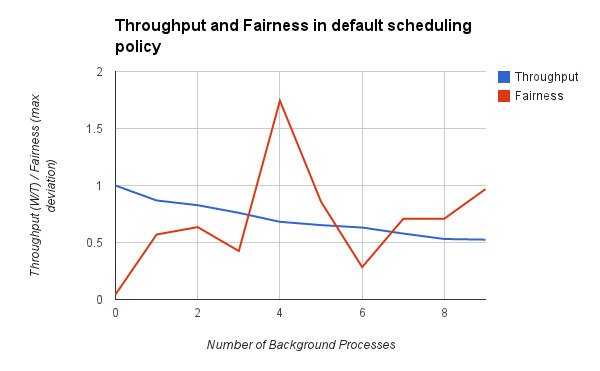
\includegraphics[width=\linewidth]{th_vs_fair.png}
  \caption{}
  \label{fig:thvsfair1}
\end{subfigure}%
\begin{subfigure}{.5\textwidth}
  \centering
  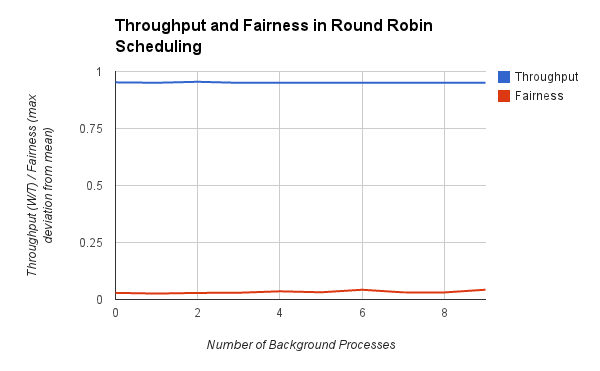
\includegraphics[width=\linewidth]{rr_th_fair.png}
  \caption{}
  \label{fig:thvsfair2}
\end{subfigure}
\caption{Throughput (higher is better) and Fairness (lower is better) with different number of background processes. (a) Default Scheduling Policy (\texttt{SCHED\_OTHER}) (b) Round Robin Scheduling Policy (\texttt{SCHED\_RR})}
\label{fig:thvsfair}
\end{figure}


%\begin{figure}[ht!]
%\centering
  %\centering
%  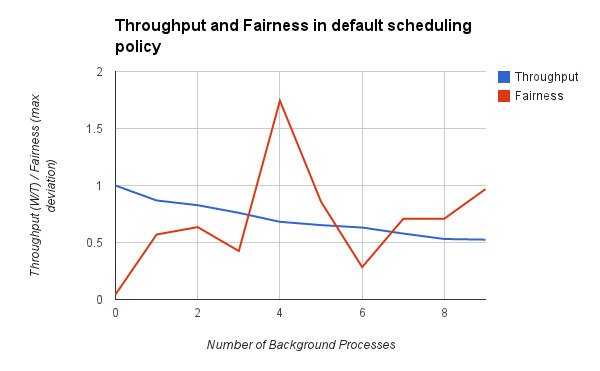
\includegraphics[width=\linewidth]{th_vs_fair.png}
%  \caption{Throughput and Fairness for 8 hashing and n background processes.}
%  \label{fig:thvsfair}
%\end{figure}

Figure \ref{fig:thvsfair1} shows that throughput decreases (in case of fixed hashing processes) as number of background processes increase which is expected since the processor is shared among more processes and less work (by hashing process) is done per unit time. However fairness is not consistent and depends on each run. The Completely Fair Scheduler(CFS) algorithm tries to run the task with the smallest \texttt{p->se.vruntime} (i.e., the task which executed least so far). Since there are number of background processes and in different runs the order in which they are executed effects the fairness among hashing threads; some of the threads can finish before the background processes and some will finish after them. In essence, if we take system as a whole CFS is quite fair. In section 5, we see how fairness and (throughput) can be increased among a group of tasks.

\section{Throughput}

\subsection{\texttt{sched\_setaffinity} }

Using \texttt{sched\_setaffinity}, we attach each hashing process to a specific CPU. CPU Affinity improves cache performance since whenever a processor adds a line to its cache, all other processors needs to invalidate the data in their cache. In certain cases there could be huge improvements in performance due to affinity. The scheduler in 2.5 exhibit excellent natural affinity and prevents bouncing of a process from one CPU to another. CPU affinity could be very effective in case data is shared among different threads (in our case there's no sharing).\\

\noindent Figure \ref{fig:cpu_affinity} shows the effect of \texttt{sched\_setaffinity} in both (8 Hashing, 8 Background) and (8 Hashing, 9 Background processes). In both cases the throughput increased by 10.9\% and 9.5\% respectively.

\begin{table}
\centering
\begin{tabular}{ |c|c|c|c|c| } 
 \hline
\textbf{Hashing Processes \#} & \textbf{Background Processes \#} & \textbf{Total Time} & \textbf{Throughput} & \textbf{max deviation from mean (fairness)}\\
\hline
8 & 8 & 15.2418 & 0.5249 & 0.7092\\ 
\hline
8 & 9 & 15.5910 & 0.5131 & 0.9686\\
\hline
\end{tabular}
\caption{Throughput for different number of background and hashing processes.}
\label{table:nvsnplusone}
\end{table}


\begin{figure}[ht!]
\centering
\begin{subfigure}{.5\textwidth}
  \centering
  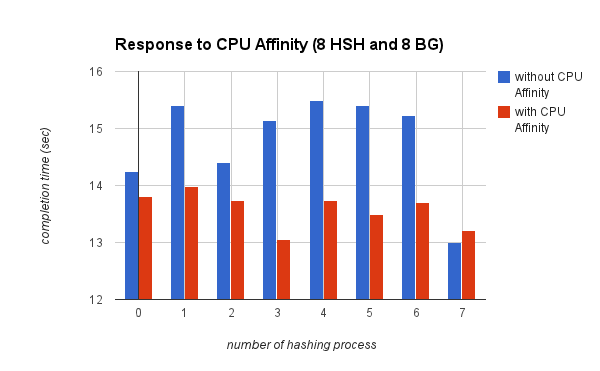
\includegraphics[width=\linewidth]{./cpu_agg_8_8.png}
  \caption{}
  \label{fig:sub1}
\end{subfigure}%
\begin{subfigure}{.5\textwidth}
  \centering
  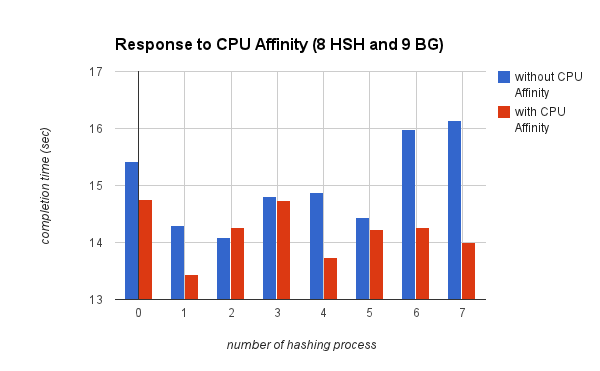
\includegraphics[width=\linewidth]{cpu_aff_8_9.png}
  \caption{}
  \label{fig:sub2}
\end{subfigure}
\caption{Response to CPU affinity: \textbf{\texttt{completion time}}  vs  \textbf{\texttt{hashing process number}}}
\label{fig:cpu_affinity}
\end{figure}

\subsection{\texttt{cgroups} }
Control Groups allow you to allocate resources - such as CPU time, system memory, network bandwidth - among user defined group of tasks (processes) running on the system. Using cgroups we can increase the amount of CPU available for hashing processes, which can significantly improve the throughput. \\

\noindent To increase \texttt{cpu.share} for hashing processes, a new cgroup for each process was created under the subsystem CPU. The \texttt{cpu.share} for all the tasks in these cgroups was increased to \texttt{2048} (default value is 1024). As a result all the hashing processes get twice the amount of cpu than other processes with default cgroups (background processes belong to default cgroups). \\

\noindent Figure \ref{fig:cgrp} (8 Hashing, 9 Background Processes) shows relative time taken by each process with and without cgroups (and sched\_affinity). \textbf{\underline{Throughput  was increased by 79.5\%}}, since the CPU was given twice to hashing processes than the background processes. It doesn't seem very useful to talk about fairness here, since we deliberately increased the CPU share and tied each hashing process to a different logical CPU.

\begin{figure}[ht!]
\centering
\begin{subfigure}{.5\textwidth}
  \centering
  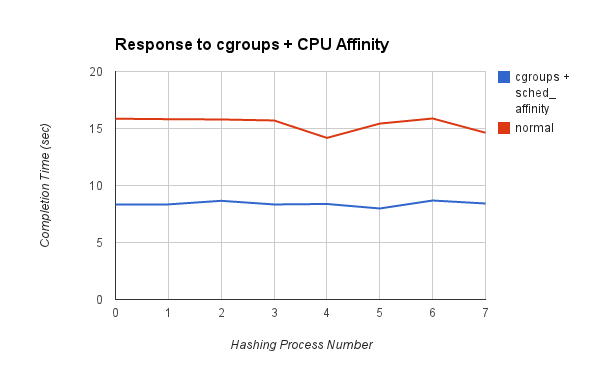
\includegraphics[width=\linewidth]{cgroup_affinity_8_9.png}
  \caption{}
  \label{fig:sub1}
\end{subfigure}%
\begin{subfigure}{.5\textwidth}
\centering

\begin{tabular}{ |c|c|c| } 
\hline
\textbf{Type} & \textbf{Total Time (sec)} & \textbf{Throughput} \\
\hline
normal & 15.5910 & 0.5131\\ 
\hline
cgroup+affinity &  8.684 & 0.9212 \\
\hline
\end{tabular}
\caption{}
\label{table:caff}
  \label{fig:sub2}
\end{subfigure}
\caption{\textbf{Response to CPU affinity + cgroups}. (a) Relative time taken by each process with and without cgroup + affinity, (b) Throughput increase of 79.5\% for cgroup + affinity}
\label{fig:cgrp}
\end{figure}

\begin{listing}[ht!]
\begin{minted}{cpp}
void computeHash(int ITERATIONS){
  for (int i = 0; i < ITERATIONS; i++) {
    if (BE_FAIR && i != 0 && i % (ITERATIONS/numProc) == 0){
      sched_yield();
    }
    /* calculate hash here */
     CityHash128(buf, 4096);
}

/* change priority and scheduling for each process to Round Robin */
inline void makeFair(int pid) {
  struct sched_param param;
  param.sched_priority = 99;
	
  if (sched_setscheduler(pid, SCHED_RR, &param) != 0) {
    perror("sched_setscheduler");
    exit(EXIT_FAILURE);
  }
}
\end{minted}
\label{lst:sched}
\caption{Implementation of scheduling policy change and voluntarily yielding.}
\end{listing}

\section{Fairness}
The default scheduler in linux - CFS (Completely Fair Scheduler) does quite a good job in scheduling fairly most of the times. However it's not always fair, in some cases the deviation from mean was a bit higher than normal. \\

\noindent One way to ensure fairness is by using Round Robin Scheduling (\texttt{SCHED\_RR}) with high priority and yielding each process after a fix number of iterations. This ensures fairness among the hashing processes in all cases. However this doesn't provide fairness among other processes (for e.g., background processes) and \emph{only root can do that.} \\

\begin{table}
\centering
\begin{tabular}{ |c|c|c|} 
 \hline
\textbf{Process Number \#} & \textbf{Total Time Taken} & \textbf{Deviation from mean (fairness)}\\
\hline
0 & 8.37 & 0.0305 \\
1 & 8.308 & 0.0315 \\
2 & 8.37 & 0.0305 \\
3 & 8.374 & 0.0345 \\
4 & 8.308 & 0.0315 \\
5 & 8.308 & 0.0315 \\
6 & 8.37 & 0.0305 \\
7 & 8.308 & 0.0315 \\
\hline 
\end{tabular}
\caption{Deviation from mean with \texttt{SCHED\_RR} scheduling policy. (8 Hashing, 9 Background Processes)}
\label{table:schedpolicy}
\end{table}

\noindent \texttt{BE\_FAIR} flag can be used to enable \texttt{SCHED\_RR} scheduling with priority of 99 (max) in the submitted code. Codeblock \texttt{1} shows the basic implementation, where \texttt{makeFair} (which changes the scheduling policy and priority) is called before initiating the compute loop. Inside the compute loop (in \texttt{computeHash} function) each hashing process voluntarily yields the processor to other hashing processes with same priority after a fixed number of iterations, hence giving fair share to all hashing processes belonging to same priority.\\

\noindent Table \ref{table:schedpolicy} shows the total time taken by each process under Round Robin scheduling (\texttt{SCHED\_RR}). \textbf{The maximum deviation from mean in this case is 0.03 compared to 0.96 with normal scheduling (\texttt{SCHED\_OTHER})}. \\

\noindent Moreover, Figure \ref{fig:thvsfair2} shows that both the throughput and Fairness are highly consistent since we have hashing processes at much higher priority than background processes. It's interesting to see that throughput is better than normal scheduling and time is fairly distributed. This is true, since our hashing processing are running at higher priority, time given to background processes is almost negligible. \\

\noindent \textbf{Minor Implementation Comment}: The branch in \texttt{computeHash}, even though will most likely be optimized by compiler in case \texttt{BE\_FAIR} is false, is still put under pre-processor so that it doesn't get generated if \texttt{BE\_FAIR} is false. This is done to keep the work constant as the compiler may do better branch prediction (Just in case) in one of the processes than other.

\section{Cryptographic vs Non-Cryptographic Hash}
A cryptographic hash function provides security guarantees that the non-cryptographic hash functions may or may not provide. Most importantly, in cryptographic hash functions, it should be hard to find collisions or pre-images. \textbf{Hard} usually means it takes very long time or is practically impossible to find collisions or pre-images. Due to these guarantees, cryptographic functions are usually slower than non-cryptographic functions. Non-cryptographic functions are usually used for CRC and 



\noindent \textbf{Time Spent on the lab \ensuremath{\approx}14 hours} 

\section{References:}
1. \url{http://www.linuxjournal.com/article/6799}  \\
2. \url{http://security.stackexchange.com/questions/11839/what-is-the-difference-between-a-hash-function-and-a-cryptographic-hash-function} \\
3. \url{http://linux.die.net/man/4/rtc} \\
4. \url{http://linux.die.net/man/4/urandom}

\end{document}